%% PolicySim — IEEE conference paper (IEEEtran, conference mode)
\documentclass[conference]{IEEEtran}
\IEEEoverridecommandlockouts
\usepackage{amsmath,amssymb,amsfonts}
\usepackage{algorithmic}
\usepackage{graphicx}
\usepackage{textcomp}
\usepackage{xcolor}
\usepackage{cite}
\usepackage{booktabs}
\usepackage{array}
\usepackage{url}
\usepackage{tikz}
\usetikzlibrary{shapes.geometric,arrows.meta,positioning,fit,backgrounds,calc}

% lightweight, robust tikz styles for block diagrams
\tikzset{
  block/.style={rectangle, rounded corners=2pt, draw=black!70, line width=0.5pt,
                fill=blue!4, align=center, inner sep=4pt, font=\footnotesize},
  store/.style={rectangle, draw=black!70, line width=0.5pt, fill=orange!8,
                align=center, inner sep=4pt, font=\footnotesize},
  lay/.style={rectangle, rounded corners=3pt, draw=black!40, dashed,
              inner sep=8pt},
  ar/.style={-{Latex[length=2mm]}, line width=0.5pt},
  arb/.style={{Latex[length=2mm]}-{Latex[length=2mm]}, line width=0.5pt}
}

\begin{document}

\title{PolicySim: Generative Agent Simulations for\\ Public-Interest Policy Evaluation}

\author{
\IEEEauthorblockN{Gowri Sankar Reddy Tatipathi}
\IEEEauthorblockA{\textit{Luddy School of Informatics,}\\
\textit{Computing, and Engineering}\\
\textit{Indiana University Bloomington}\\
Bloomington, IN, USA\\
gotati@iu.edu}
\and
\IEEEauthorblockN{Jasmine Christopher}
\IEEEauthorblockA{\textit{Luddy School of Informatics,}\\
\textit{Computing, and Engineering}\\
\textit{Indiana University Bloomington}\\
Bloomington, IN, USA\\
jaschri@iu.edu}
\and
\IEEEauthorblockN{Uday Vallabhaneni}
\IEEEauthorblockA{\textit{Luddy School of Informatics,}\\
\textit{Computing, and Engineering}\\
\textit{Indiana University Bloomington}\\
Bloomington, IN, USA\\
udvall@iu.edu}
}

\maketitle

\begin{abstract}
Deciding how to design a public program is hard because the outcome depends on people: on how they read a rule, whether they trust the institution behind it, and how their choices ripple through a community. The methods normally used to study a policy before it launches, such as rule-based agent simulations, econometric models, and surveys, are good at summarizing averages or encoding fixed behavior, but they say little about the reasoning, confusion, mistrust, and social pressure that often decide whether a policy works. This paper introduces \textbf{PolicySim}, which we frame as a \emph{trustworthy generative social digital twin} for policy experimentation. In it, each resident of a virtual community is a software agent whose decisions are produced by a Large Language Model (LLM) reasoning over a personal profile, a memory of past events, a set of evolving beliefs, and a position in a social network. A policy written in ordinary language is translated into the rules of the simulation; the agents then perceive their circumstances, recall what is relevant, decide, and influence one another, so that community-level effects emerge from these interactions. Our contributions are a generative-agent framework for policy analysis, a six-layer cognitive and social architecture, an evaluation approach built on historical backtesting together with fairness, fidelity, and reality-alignment metrics, and a human-centered design in which every result carries an estimate of how far it can be trusted. We are careful to separate what is proposed, what is hypothesized, and what still needs testing: the central claim, that LLM-driven agents predict population responses better than classical baselines, is stated as a falsifiable hypothesis with a matching experimental plan. We also keep the documented failure modes of LLM-based simulation in view, so that PolicySim is presented as accountable decision support rather than automated policymaking.
\end{abstract}

\begin{IEEEkeywords}
Generative AI, large language models, multi-agent systems, agent-based modeling, computational social science, public-interest technology, responsible AI, decision support
\end{IEEEkeywords}

\section{Introduction}

\subsection{Background}
Over the past few years, generative artificial intelligence built on Large Language Models (LLMs) has moved quickly from the laboratory into everyday use across science, business, and government. An LLM is a neural network trained on very large amounts of text to predict the next word, and a striking side effect of that simple objective is an ability to carry out tasks that look like reasoning when the model is prompted well. As these systems shift from answering questions to taking actions inside larger software, a question becomes natural for the public sector: could they help us anticipate how a policy will land on real people before it is put into effect?

This question matters because public decisions are, at heart, decisions about people. A local health department or a housing nonprofit usually works with a small budget and has no ethical way to run a controlled experiment on the families it serves. When a program is designed badly, the cost falls on exactly the people it was meant to help. What such organizations need, then, is not only a way to forecast outcomes but a way to do so responsibly: a tool that broadens their view of what might happen while leaving final judgment and accountability with people.

\subsection{Problem}
Before committing to a policy, an organization usually wants to understand three things. The first is who benefits and who is left out. The second is how behavior will actually change: whether people will take up a benefit, alter a daily routine, or believe an official message. The third is what will go wrong in ways that surface only in practice. A program that looks sound on paper can still fail because its application form discourages the very households it targets, because a payment arrives out of step with the rent cycle, or because a single bad experience spreads distrust through a neighborhood and quietly suppresses participation. These are failures of understanding, communication, and social structure rather than of arithmetic, and they are precisely what conventional quantitative tools tend to miss.

\subsection{Research gap}
Four broad families of methods are used to study a policy in advance, and each runs into the same wall. \emph{Agent-based models} (ABMs) simulate a population of individuals who follow hand-written rules and interact, so that large-scale patterns grow out of local behavior~\cite{schelling1971,epstein1996}. Each agent is essentially a small program of the form \texttt{if condition then action}. ABMs capture diversity and emergence well, but every behavior has to be specified by the modeler in advance, and the agents cannot read meaning from a confusing letter or a rumor. \emph{Econometric and other statistical models} estimate relationships from historical data and project them forward; they are rigorous, yet they assume behavior stays stable when the policy regime changes and they average away the individual differences in which unequal impacts actually live. \emph{Surveys} ask people directly, but respondents are notoriously poor at predicting their own behavior under unfamiliar conditions, and reaching vulnerable groups is slow and costly. \emph{Static prediction models} learn a mapping from inputs to an outcome but cannot show how that outcome is produced through interaction over time.

The shared shortcoming can be put in a single line:
\begin{quote}
\emph{Existing systems simulate actions well, but struggle to simulate human reasoning and adaptation.}
\end{quote}
Whether a policy succeeds depends mostly on things that sit between the individual action and the population average: how a rule is understood, whether an agency is trusted, and what one's neighbors are seen to do. A method whose basic unit is the action, or the aggregate, can reproduce the consequences of reasoning when history repeats itself, but it cannot represent the reasoning, and so it cannot extend to genuinely new policies, where the human response is exactly the unknown.

\subsection{From fixed rules to simulated reasoning}
This shortcoming points to a change in the agent itself. A classical simulation runs along a fixed track,
\begin{center}
\textit{Rules} $\rightarrow$ \textit{Actions} $\rightarrow$ \textit{Outcomes},
\end{center}
where the modeler writes the decision rules ahead of time, the agents carry them out, and the aggregate result follows. Human behavior, though, resists being pinned down by fixed rules. The same situation means different things to different people; we act on incomplete information, change our minds with circumstance, and take our cues from those around us. These features are easy to overlook and hard to list in full, which is why rule-based models tend to fail on the soft frictions that decide a policy's fate.

Large Language Models suggest a different route. Having been trained on an enormous range of human writing, an LLM carries a broad sense of how a person in a given situation might think and act. Placed inside an agent and given a detailed persona and context, it can interpret new, language-based information and respond in ways no one wrote down in advance. PolicySim therefore runs along a longer track,
\begin{center}
\textit{Perception} $\rightarrow$ \textit{Memory} $\rightarrow$ \textit{Reasoning} $\rightarrow$ \textit{Decision} $\rightarrow$ \textit{Interaction} $\rightarrow$ \textit{Emergent Society},
\end{center}
in which an agent notices its situation, draws on memory, weighs its options, decides, and then acts on and reacts to others through a social network, so that the shape of the whole community emerges from many small interactions rather than from a single rule. This is the paper's central idea. Seen this way, PolicySim is more than a simulator: it is a trustworthy generative social digital twin for policy experimentation, a working model of a community that brings together LLM reasoning, agent memory, social interaction, counterfactual comparison of policies, and responsible-AI validation. Building that combination, and being honest about how far it can be trusted, is what this work sets out to do.

The motivation for public-interest organizations is concrete. They serve people with little margin for error, they operate under real budget limits, and they cannot experiment on actual communities. A tool that lets them try a policy on a synthetic community, watch where friction and inequity appear, and adjust the design before launch is valuable precisely because, in the real world, the cost of getting it wrong falls on those least able to absorb it.

\subsection{Contribution}
To address this gap, we develop PolicySim, the trustworthy generative social digital twin sketched above. The paper makes five contributions:
\begin{enumerate}
\item \textbf{A generative-agent simulation framework for policy analysis}, in which LLM-driven agents reason about, and respond to, plain-language policy proposals in a virtual community grounded in real demographic data.
\item \textbf{A six-layer cognitive-social digital twin architecture}, spanning policy understanding, synthetic population generation, agent cognition, social intelligence, world simulation with counterfactual reasoning, and responsible-AI validation.
\item \textbf{A responsible-AI evaluation framework}, centered on historical backtesting against recorded outcomes and on fairness/fidelity auditing designed to detect the known failure modes of LLM-based social simulation.
\item \textbf{A human-centered decision-support approach}, in which every result carries an explicit estimate of how far it can be trusted, and the system is designed to assist - never replace - human policymakers.
\item \textbf{New validation metrics}, including an Agent Behavioral Fidelity Score and a system-level Simulation Reality Alignment Score that combine prediction accuracy, behavioral realism, fairness, and uncertainty calibration.
\end{enumerate}
Throughout, we keep three categories distinct: what we \emph{propose} (the framework and its architecture), what we \emph{hypothesize} (that the approach will outperform classical baselines on outcomes driven by cognition), and what still requires \emph{validation} (the experiments described in Sections~\ref{sec:eval} and~\ref{sec:expdesign}). We do not report validated results, and we say so plainly wherever it matters.

\section{Related Work}

\subsection{Agent-based modeling and its ceiling}
Agent-based modeling has a long and productive history in the social sciences. Schelling showed that mild individual preferences about one's neighbors can tip an entire city into segregation~\cite{schelling1971}, and Epstein and Axtell's \emph{Sugarscape} set the ``generative'' benchmark of explaining a social pattern by growing it from the bottom up~\cite{epstein1996}. The agents in these models reason through explicit logic: state machines, decision trees, or simple utility rules. The approach is excellent for studying how local choices add up, and it remains in wide use. Its ceiling comes from two sources. First, realism is limited by how much the modeler can foresee and encode by hand, which leaves the model fragile in situations its author never imagined. Second, the agents respond to numbers, not to meaning: they cannot read a badly worded notice or make sense of a rumor.

\subsection{Putting a language model inside the agent}
A recent line of work replaces the rule engine with an LLM. Park and colleagues introduced \emph{generative agents}, LLM-driven characters with memory, reflection, and planning that behaved believably both alone and together in a small simulated town~\cite{park2023}. Three of their ideas carry over to PolicySim. Memory keeps natural-language records of what an agent has experienced, separating specific events from the general lessons drawn from them. Reasoning is supplied by the LLM and is often drawn out step by step through chain-of-thought prompting~\cite{wei2022}. Planning lets the agent set goals and order its actions sensibly over time, with the reason-and-act loop of ReAct~\cite{yao2023} and the self-review of Reflexion~\cite{shinn2023} as typical mechanisms. DeepMind's Concordia turned these ideas into a general library for generative agent-based modeling, using a central referee to ground what agents do in a shared world~\cite{vezhnevets2023}, and later systems have scaled the approach to thousands or even millions of agents~\cite{piao2025,gao2024}.

\subsection{How faithfully can a model stand in for people?}
A parallel literature asks whether LLMs can actually represent human social behavior. Argyle and colleagues proposed the idea of \emph{algorithmic fidelity}: conditioning a model on a person's background can make its answers resemble those of the matching group, which suggests that LLMs hold fine-grained, demographically structured patterns rather than one flat bias~\cite{argyle2023}. Park and colleagues pushed this further, building agents from interviews with more than a thousand real people; the agents reproduced participants' survey answers about as well as the participants did themselves two weeks later, and, notably, narrowed the accuracy gaps between racial and ideological groups that thin demographic labels tend to leave behind~\cite{park2024}.

\subsection{Promise and peril for the public interest}
AI is increasingly used to support nonprofits and public services, from triaging needs to designing programs. The appeal is a low-cost laboratory in which an intervention can be rehearsed before it touches anyone. The danger, well documented in the same literature, is that fluent output invites misplaced confidence. Several studies show that simulated populations can distort as much as they inform: Bisbee and colleagues found that LLM-generated survey responses exaggerated political polarization by roughly a factor of seven through stereotype amplification~\cite{bisbee2024}; Pataranutaporn and colleagues reported systematic errors when estimating well-being across 64{,}000 people in 64 countries~\cite{pataranutaporn2025}; and Santurkar and colleagues showed that a model's default ``opinions'' over-represent some groups while under-representing others~\cite{santurkar2023}.

\subsection{Where PolicySim fits}
Table~\ref{tab:compare} places PolicySim against these alternatives. The generative-agent literature has mostly settled \emph{that} LLM agents can behave believably. PolicySim takes up a narrower and, we think, more pressing question: \emph{whether, and how far, that believability can be turned into policy advice that is accountable}. What sets it apart is a validation-first stance built on historical backtesting and fairness auditing, a population assembled only from public data and tied to a specific locality, and a design that reports the trustworthiness of every result. We do not claim to build the largest or most lifelike artificial society; we propose a way to measure and govern one so that it can be used safely in public decisions.

\begin{table}[!t]
\caption{PolicySim and Existing Simulation Approaches}
\label{tab:compare}
\centering
\renewcommand{\arraystretch}{1.25}
\footnotesize
\begin{tabular}{@{}p{1.2cm}p{1.55cm}p{1.65cm}p{1.9cm}@{}}
\toprule
\textbf{Approach} & \textbf{Strength} & \textbf{Limitation} & \textbf{PolicySim advantage} \\
\midrule
Rule-based ABM & Heterogeneity and emergence & Hand-coded rules; no language understanding & Agents reason over language, not fixed rules \\
Econometric models & Statistical rigor on past data & Assume stable behavior; average away individuals & Models individual reasoning and change \\
Survey prediction & Direct human input & Hypothetical bias; costly; weak self-forecasts & Simulates behavior under new, untried policies \\
Generative agent simulation & Believable individual behavior & Believability not yet shown to be accurate & Adds validation, fairness, and trust calibration \\
\bottomrule
\end{tabular}
\end{table}

\section{The PolicySim Framework}

At its simplest, PolicySim is a way of turning a policy into a range of likely consequences (Fig.~\ref{fig:flow}). It builds a virtual community in which software agents stand in for different residents and stakeholders, lets them live through a proposed policy, and reports what happens. The framework can be read in three stages.

\textbf{Input: a policy in plain language.} The starting point is a proposal written the way a policymaker would actually write it, for example, \emph{``Increase public-transportation subsidies for low-income riders by 50\%.''} No code is required.

\textbf{Processing: agents reason and interact.} A dedicated agent first converts the proposal into concrete simulation settings, deciding who qualifies, by how much, and on what schedule. The population of citizen agents then moves forward under the new policy: each agent looks at its own situation, recalls what is relevant, decides what to do, and acts. Because the agents are linked in a social network, attitudes and information pass between them, and collective patterns build up over time.

\textbf{Output: social, economic, and behavioral effects.} The framework reports the patterns that emerge, such as take-up rates, shifts in the distribution of income or transit use, and gaps between demographic groups, alongside sample agent reasoning that shows \emph{why} a given outcome appeared. Every result is reported together with an estimate of how far it can be trusted for the policy at hand (Section~\ref{sec:resp}).

\begin{figure*}[!t]
\centering
\resizebox{\textwidth}{!}{%
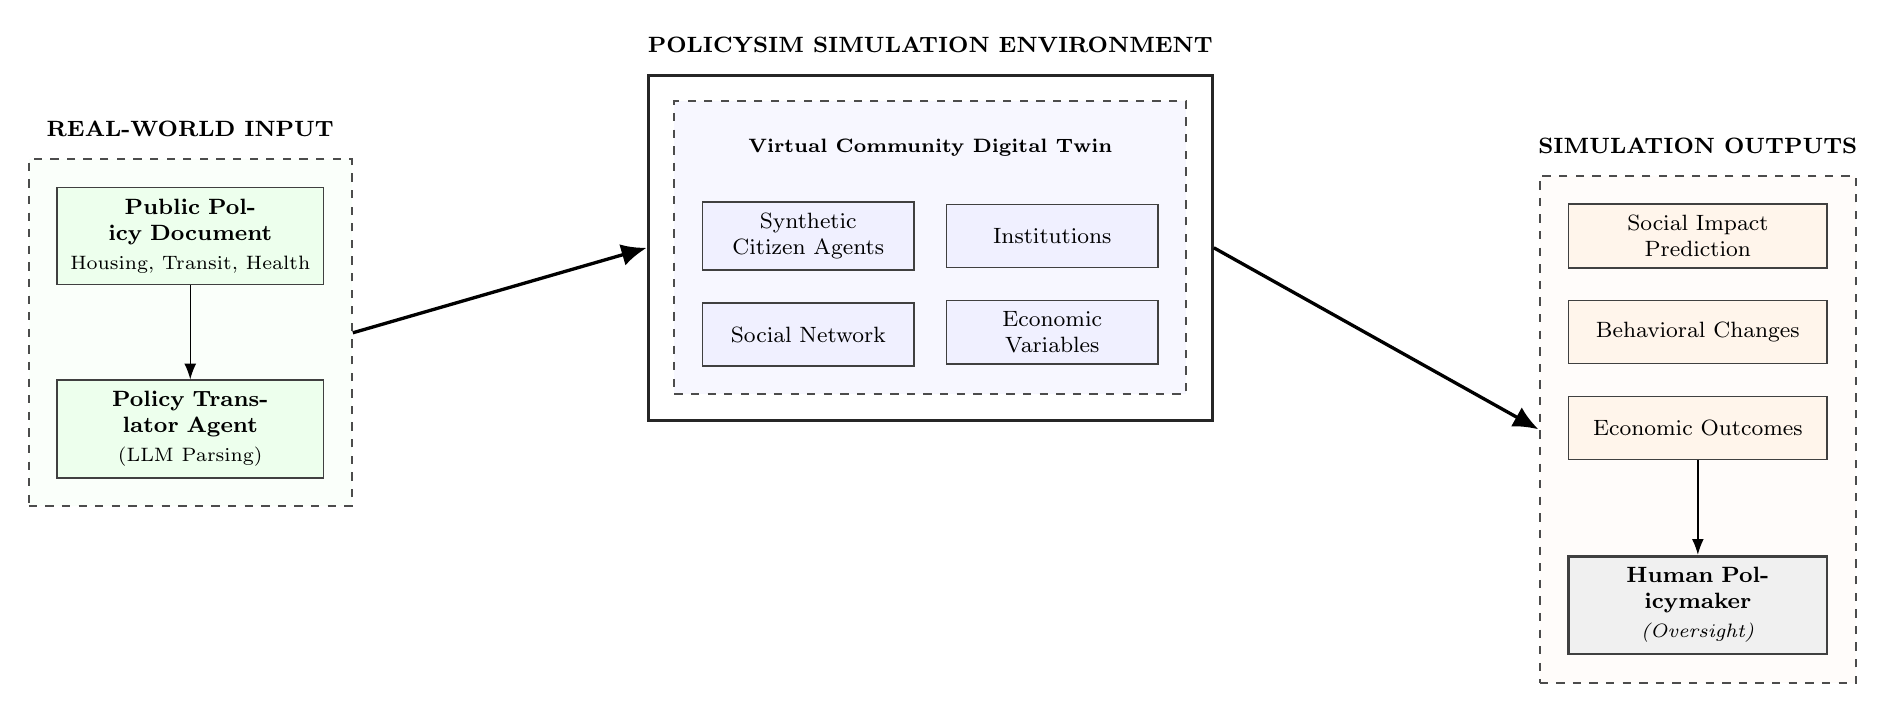
\begin{tikzpicture}[
  font=\footnotesize,
  inode/.style={rectangle, draw=black!75, line width=0.5pt, fill=white, align=center,
                inner sep=4pt, minimum height=8mm, font=\footnotesize},
  dpanel/.style={rectangle, draw=black!70, dashed, line width=0.8pt, inner sep=10pt},
  spanel/.style={rectangle, draw=black!85, line width=1.2pt, inner sep=9pt},
  ptitle/.style={font=\footnotesize\bfseries},
  bigar/.style={-{Latex[length=3.2mm,width=2.8mm]}, line width=1.2pt}
]
% ---- LEFT: Real-World Input ----
\node[inode, fill=green!7, text width=3.1cm] (doc) {\textbf{Public Policy Document}\\[1pt]{\scriptsize Housing, Transit, Health}};
\node[inode, fill=green!7, text width=3.1cm, below=12mm of doc] (trans) {\textbf{Policy Translator Agent}\\[1pt]{\scriptsize (LLM Parsing)}};
\draw[ar] (doc) -- (trans);
\begin{scope}[on background layer]
\node[dpanel, fill=green!2, fit=(doc)(trans)] (leftP) {};
\end{scope}
\node[ptitle, above=1.5mm of leftP.north] {REAL-WORLD INPUT};
% ---- CENTER: Simulation Environment > Digital Twin ----
\node[inode, fill=blue!6, text width=2.4cm, right=48mm of doc] (cit) {Synthetic Citizen Agents};
\node[inode, fill=blue!6, text width=2.4cm, right=4mm of cit] (inst) {Institutions};
\node[inode, fill=blue!6, text width=2.4cm, below=4mm of cit] (soc) {Social Network};
\node[inode, fill=blue!6, text width=2.4cm, below=4mm of inst] (econ) {Economic Variables};
\node[font=\scriptsize\bfseries] (twintitle) at ([yshift=7mm]$(cit.north)!0.5!(inst.north)$) {Virtual Community Digital Twin};
\begin{scope}[on background layer]
\node[dpanel, fill=blue!3, fit=(cit)(inst)(soc)(econ)(twintitle)] (twin) {};
\node[spanel, fit=(twin)] (centerP) {};
\end{scope}
\node[ptitle, above=1.5mm of centerP.north] {POLICYSIM SIMULATION ENVIRONMENT};
% ---- RIGHT: Outputs ----
\node[inode, fill=orange!8, text width=3.0cm, right=52mm of inst] (o1) {Social Impact Prediction};
\node[inode, fill=orange!8, text width=3.0cm, below=4mm of o1] (o2) {Behavioral Changes};
\node[inode, fill=orange!8, text width=3.0cm, below=4mm of o2] (o3) {Economic Outcomes};
\node[inode, fill=gray!12, line width=1pt, text width=3.0cm, below=12mm of o3] (pm) {\textbf{Human Policymaker}\\[1pt]{\scriptsize \emph{(Oversight)}}};
\draw[ar] (o3) -- (pm);
\begin{scope}[on background layer]
\node[dpanel, fill=orange!2, fit=(o1)(o2)(o3)(pm)] (rightP) {};
\end{scope}
\node[ptitle, above=1.5mm of rightP.north] {SIMULATION OUTPUTS};
% ---- inter-panel arrows ----
\draw[bigar] (leftP.east) -- (centerP.west);
\draw[bigar] (centerP.east) -- (rightP.west);
\end{tikzpicture}%
}
\caption{PolicySim overall research framework. A natural-language policy document is parsed by the Policy Translator Agent and injected into a generative-agent simulation over a virtual community digital twin (synthetic citizen agents, a social network, institutions, and economic variables); the framework reports social, behavioral, and economic outcomes under human policymaker oversight.}
\label{fig:flow}
\end{figure*}

\section{Language Model Foundations for Generative Policy Agents}
\label{sec:llm}

PolicySim depends on the ability of a Large Language Model to read a description of a situation and produce a coherent, context-appropriate response. This section reviews the parts of the underlying \emph{transformer} architecture that make this possible, and links each part to its role in the simulation. We keep the treatment compact and explain each term before using it. The architecture itself is standard~\cite{vaswani2017}; our contribution lies in how it is composed into a policy-simulation system, not in the architecture.

\subsection{Tokens and embeddings}
A language model does not operate on raw text. The input is first split into \emph{tokens} (words or word fragments), and each token is mapped to a vector of real numbers called an \emph{embedding}. Embeddings place tokens with related meanings near one another in a high-dimensional space, which gives the model a numerical representation it can compute with. The same idea reappears in PolicySim at the level of memory: an agent's experiences are stored as embeddings so that a current situation can retrieve semantically similar past events (Section~\ref{sec:adapt}).

\subsection{Encoder, decoder, and self-attention}
The original transformer has an \emph{encoder} that reads an input sequence into a set of representations and a \emph{decoder} that generates an output sequence from them. The language models used in PolicySim are decoder-style models that generate text one token at a time, each new token conditioned on all previous ones. The mechanism that makes this work is \emph{self-attention}, which lets the model weigh the relevance of every token to every other token when forming a representation. Each token produces three vectors: a query $Q$, a key $K$, and a value $V$. The attention output is
\begin{equation}
\mathrm{Attention}(Q,K,V) = \mathrm{softmax}\!\left(\frac{QK^{\top}}{\sqrt{d_k}}\right)V,
\end{equation}
where $d_k$ is the dimension of the key vectors and the factor $\sqrt{d_k}$ keeps the dot products in a stable range. Intuitively, $QK^{\top}$ measures how well each query matches each key; the softmax turns these scores into weights that sum to one; and the result is a weighted average of the value vectors. The effect is that, when the model processes a word, it can attend to the other words that give it meaning. This is exactly the property PolicySim needs: an agent's decision must depend on the whole of its situation - its constraints, the policy text, and the relevant memories - rather than on any single phrase in isolation.

\subsection{Multi-head attention and positional encoding}
A single attention operation captures one kind of relationship. \emph{Multi-head attention} runs several attention operations in parallel, each with its own learned projections, and concatenates the results before a final linear projection. Different heads can specialize; one may track who is speaking while another tracks time or quantity. Because attention itself ignores word order, the model also adds a \emph{positional encoding} to each token embedding - typically a pattern of sinusoids of different frequencies - so that the position of a token in the sequence is represented. Order matters for PolicySim because the sequence of events in an agent's life, such as what happened first, what came due, and what was learned, changes the decision.

\subsection{From architecture to context understanding}
Stacking many multi-head-attention and feed-forward layers produces a model that, given a sequence of tokens, predicts the next one. Trained at scale, this simple objective yields a system that can follow instructions, answer questions, and continue a described situation in a human-like way~\cite{brown2020}. For our purposes the key consequence is that a transformer can integrate a long, qualitative context - a persona, a financial constraint, a policy notice, and a set of memories - into a single coherent decision. This is the capability that hand-coded agent rules lack, and it is the foundation on which the rest of PolicySim is built.

\section{Domain-Specific Language Model Adaptation}
\label{sec:adapt}

PolicySim does not train a language model from scratch. Doing so would require resources far beyond any public-interest setting and would discard the general knowledge that makes the agents useful. Instead, we start from an existing open foundation model - for example a model in the Llama~\cite{touvron2023} or Mistral~\cite{jiang2023} families, or a comparable GPT-style model - and adapt it to the policy-simulation domain through a staged pipeline:
\begin{enumerate}
\item a pre-trained foundation model provides general language and reasoning ability;
\item domain knowledge (local institutions, program rules, community context) is integrated;
\item retrieval-augmented generation grounds responses in specific documents;
\item instruction tuning shapes the model to follow the simulation's task format;
\item agent-specific prompting assigns each agent its persona and constraints; and
\item evaluation and alignment check that behavior is realistic and safe.
\end{enumerate}
The subsections below describe the main techniques. Throughout, these are the \emph{intended} adaptation methods; their effect on simulation fidelity is an empirical question addressed in Sections~\ref{sec:eval} and~\ref{sec:expdesign}.

\subsection{Fine-tuning}
\emph{Fine-tuning} continues training a pre-trained model on a smaller, task-specific dataset so that its parameters shift toward the target domain. For language generation the standard objective is the cross-entropy (negative log-likelihood) loss, which rewards the model for assigning high probability to the correct next token given the preceding context. Minimizing it makes the model favor the desired continuations. In PolicySim, fine-tuning is the route by which citizen agents can be \emph{calibrated} toward real behavioral data (for example, observed program take-up patterns), which is the most direct way to improve realism; we use it cautiously to avoid overfitting that would erase the model's general reasoning.

\subsection{Parameter-efficient fine-tuning (LoRA)}
Updating all parameters of a large model is expensive and produces a full copy of the model for every variant. \emph{Low-Rank Adaptation} (LoRA) avoids this by freezing the original weights $W_0$ and learning a small low-rank update,
\begin{equation}
W = W_0 + \Delta W = W_0 + BA, \qquad B \in \mathbb{R}^{d\times r},\; A \in \mathbb{R}^{r\times k},
\end{equation}
where the rank $r$ is much smaller than the weight dimensions, so the number of trainable parameters drops by orders of magnitude~\cite{hu2022}. This is practical for PolicySim for two reasons: it brings adaptation within reach of modest hardware, and it makes it cheap to maintain several lightweight adapters - for instance, one tuned for a particular locality or policy domain - on top of a single shared base model.

\subsection{Prompt engineering}
Not all adaptation requires training. \emph{Prompt engineering} shapes behavior through the text given to the model at run time. We rely on three patterns. \emph{Role prompting} assigns the model an identity (``you are a 34-year-old single parent in Zone~B''), which conditions its responses on that persona. \emph{Context injection} supplies the current situation and retrieved memories so the decision is grounded in the agent's circumstances. \emph{Constraint-based prompting} states hard limits - available cash, a deadline, and the set of allowed actions - so that responses stay feasible. Together these patterns turn one base model into a population of distinct agents without separate training for each.

\subsection{Retrieval-augmented generation}
\emph{Retrieval-Augmented Generation} (RAG) supplies the model with relevant external information at run time rather than relying only on its trained parameters~\cite{lewis2020}. The pipeline has three steps: documents (and, in our case, agent memories) are converted into embeddings and stored; a query - the agent's current situation - is embedded and used to retrieve the most similar items, where similarity is measured by the cosine of the angle between the query and stored vectors; and the retrieved text is injected into the prompt as additional context. Retrieval also serves a practical purpose: because a model can attend only to a bounded \emph{context window}, retrieval selects the few most relevant items to place in that limited space rather than overflowing it. RAG plays two roles in PolicySim. It grounds the policy-translation step in the actual wording of a regulation, which reduces invention, and it implements agent memory by retrieving the experiences most relevant to the present moment.

\section{Alignment and Behavioral Optimization of PolicySim Agents}
\label{sec:align}

Adaptation makes the agents capable; \emph{alignment} makes them behave in ways that are useful and safe. The standard technique is Reinforcement Learning from Human Feedback (RLHF), which proceeds in three stages:
\begin{center}
\textit{Human feedback} $\rightarrow$ \textit{Reward model} $\rightarrow$ \textit{Policy optimization}.
\end{center}
People compare model outputs and indicate which is better; these comparisons train a \emph{reward model} that predicts human preference; and the language model is then optimized to produce outputs the reward model scores highly~\cite{christiano2017,ouyang2022}. The optimization step is commonly carried out with Proximal Policy Optimization (PPO).

\subsection{Proximal policy optimization}
PPO is a reinforcement-learning algorithm that improves a policy while preventing it from changing too much in a single update, which keeps training stable~\cite{schulman2017}. Let $r_t(\theta) = \pi_\theta(a_t\mid s_t)/\pi_{\theta_{\text{old}}}(a_t\mid s_t)$ be the ratio between the new and old policies for action $a_t$ in state $s_t$, and let $\hat{A}_t$ estimate how much better that action was than expected (the advantage). PPO maximizes the clipped objective
\begin{equation}
\mathcal{L}^{\mathrm{CLIP}}(\theta) = \mathbb{E}_t\!\left[\min\!\big(r_t(\theta)\hat{A}_t,\; \mathrm{clip}(r_t(\theta), 1-\epsilon, 1+\epsilon)\,\hat{A}_t\big)\right],
\end{equation}
where $\epsilon$ is a small constant. The clip term removes the incentive to push the policy beyond the trust region $[1-\epsilon, 1+\epsilon]$, so improvements are made in small, stable steps.

\subsection{What alignment should and should not do in PolicySim}
Alignment must be applied with care in a simulation whose purpose is realism, and we draw an explicit distinction. For the \emph{system agents} - the policy translator and the report writer - alignment is straightforwardly beneficial: it makes them follow instructions, stay grounded in the provided text, respect the output format, and avoid harmful or unsupported statements. For the \emph{citizen agents}, however, the goal is not to make them obedient or uniform. Real residents do not always follow rules or behave well, and optimizing citizen agents toward a notion of good behavior would remove the diversity and friction the simulation exists to capture. We therefore restrict citizen-agent optimization to two safe purposes: keeping outputs within hard feasibility and safety constraints (an agent cannot spend money it does not have, and must not produce harmful content), and improving the \emph{consistency} of an agent with its own established persona over time. Improving citizen \emph{realism} is treated as a calibration problem (fine-tuning against behavioral data, Section~\ref{sec:adapt}), not an alignment problem. This separation keeps alignment from quietly degrading the realism of the simulation, and it is itself a claim we would test rather than assume.

\section{Advanced Agent Reasoning Techniques}
\label{sec:techniques}

Beyond the base model, several established techniques improve how an agent thinks and acts. We summarize the ones PolicySim uses and explain the role of each. \emph{Chain-of-thought reasoning} prompts the model to lay out intermediate steps before committing to an answer, which improves performance on multi-step problems~\cite{wei2022}; in PolicySim it produces a short rationale for each decision, which also makes the decision auditable. \emph{ReAct} interleaves reasoning with actions, so an agent can think, take a step, observe the result, and think again~\cite{yao2023}; this matches the simulation loop, where an agent must react to a changing world. \emph{Reflection} lets an agent review recent experience and update its beliefs~\cite{shinn2023}; this is how trust in an institution grows or decays over a run. \emph{Tool calling} and \emph{function calling} let an agent invoke external operations through a defined interface, which in PolicySim is how an agent commits a validated, structured action to the simulation engine rather than emitting free text. \emph{Memory augmentation} extends the agent beyond its limited context window by storing and retrieving past experiences, giving it continuity across a long simulation. \emph{Planning} lets an agent sequence intended activities over time so its behavior is coherent rather than short-sighted. \emph{Self-correction} allows an agent to detect and repair an infeasible or ill-formed action before it is executed, improving robustness. Finally, \emph{retrieval augmentation} (Section~\ref{sec:adapt}) keeps both reasoning and memory grounded in relevant, specific information. None of these techniques is novel on its own; the contribution is their disciplined combination inside a single, auditable agent built for policy simulation.

\section{System Architecture}
\label{sec:arch}

PolicySim uses a three-layer, decoupled architecture (Fig.~\ref{fig:arch}): a frontend for human interaction, a backend that runs the simulation, and an AI layer that supplies cognition, knowledge, memory, and social structure. Decoupling lets the expensive part (AI inference) scale independently of the user interface.

\subsection{Frontend layer}
The frontend is the experiment console for a policymaker. It provides a \emph{user dashboard} that summarizes outcomes; a \emph{policy-input} interface for writing a proposal and configuring a scenario; and \emph{simulation visualization} that shows results on a real map of the community and as live charts of macro-indicators as simulated time advances. A distinctive feature is the ability to inspect an individual agent's reasoning trace, so a user can interrogate \emph{why} a result occurred rather than only \emph{that} it did - a requirement for the trust-calibration goal of Section~\ref{sec:resp}.

\subsection{Backend layer}
The backend is the control plane. Its \emph{simulation engine} owns the global clock and advances the world one step at a time. \emph{Agent orchestration} distributes the agents' reasoning across parallel workers and collects their actions. \emph{API communication} exposes the engine to the frontend and streams live telemetry. The control plane deliberately stays ``thin'' - it coordinates and persists, but does not itself perform cognition, which is delegated to the AI layer so that it can be scaled separately.

\subsection{AI layer}
Four components give the agents their capabilities.

\emph{Large Language Models} are the reasoning core: given a description of an agent and its situation, the LLM generates the agent's decision. Most agents use a smaller, efficient open model; a few system tasks use a larger model (Section~\ref{sec:impl}).

\emph{Retrieval-Augmented Generation (RAG)} grounds the LLM in specific knowledge. RAG is a technique that retrieves relevant documents from an external store and supplies them to the LLM, so its output reflects that knowledge rather than only its trained parameters. In PolicySim, RAG grounds the policy-translation step in the actual text of the policy and relevant rules.

\emph{A vector database} provides agent memory. A vector database stores text as numeric ``embedding'' vectors - representations in which similar meanings are nearby - and retrieves items by semantic similarity rather than exact keywords. Each agent's episodic memories live here and are recalled by similarity to the agent's current situation.

\emph{A knowledge graph} (graph database) stores the social structure. A graph database represents entities as nodes and relationships as edges, making it efficient to ask who is connected to whom and how strongly. PolicySim uses it for households, workplaces, neighborhood ties, and trust between agents, so that social influence and information spread are first-class.

\subsection{AI orchestration}
Above these components sits an orchestration layer that coordinates many agents efficiently. An \emph{agent manager} tracks the state of each agent and decides which agents act in a given step; \emph{task scheduling} places the resulting reasoning calls onto the worker pool and balances load; \emph{model routing} sends each call to the appropriate model - a small model for routine citizen decisions and a larger model for demanding tasks; and \emph{context management} assembles the prompt for each call, combining the agent's persona, current situation, and retrieved memories while staying within the model's context window. Orchestration is what allows a single shared infrastructure to run thousands of agents without manual coordination.

\subsection{Memory architecture}
PolicySim distinguishes several kinds of memory, mirroring human memory and matching each to suitable storage. \emph{Short-term memory} holds the current situation and the last few steps in the model's context. \emph{Episodic memory} records specific, time-stamped experiences and is stored as embeddings in the vector database. \emph{Long-term memory} holds beliefs and generalizations distilled from experience through reflection. \emph{Semantic memory} holds stable background knowledge about the world and its institutions. Separating these types lets the system retrieve the right kind of information for a given decision and keeps the active context small.

\subsection{Model serving}
Running thousands of agents is feasible only with careful model serving. A \emph{small open model} handles the many routine decisions of citizen agents, where speed and cost dominate; a \emph{larger model} is reserved for a few demanding tasks - policy translation, report writing, and complex reasoning - where quality matters more than volume. Serving the small model with an efficient inference engine, and reserving the large model for rare calls, gives a favorable cost--performance balance: the dominant cost term stays small while quality is preserved where it counts.

\begin{table}[!t]
\caption{PolicySim Architecture Components vs.\ Traditional Approaches}
\label{tab:archcompare}
\centering
\renewcommand{\arraystretch}{1.25}
\footnotesize
\begin{tabular}{@{}p{1.6cm}p{1.55cm}p{1.5cm}p{1.7cm}@{}}
\toprule
\textbf{Component} & \textbf{Traditional ABM} & \textbf{Econometric} & \textbf{PolicySim} \\
\midrule
Agent reasoning & Fixed rules & None (aggregate) & LLM reasoning \\
Memory & None or scalar & None & Episodic + long-term \\
Social interaction & Simple rules & Absent & Trust-weighted network \\
Language understanding & None & None & Native \\
Policy adaptation & Manual recoding & Re-estimation & Language translation \\
Explainability & Rule trace & Coefficients & Reasoning traces \\
Uncertainty & Rare & Confidence intervals & Seed/model ensembles \\
\bottomrule
\end{tabular}
\end{table}

\begin{figure*}[!t]
\centering
\resizebox{\textwidth}{!}{%
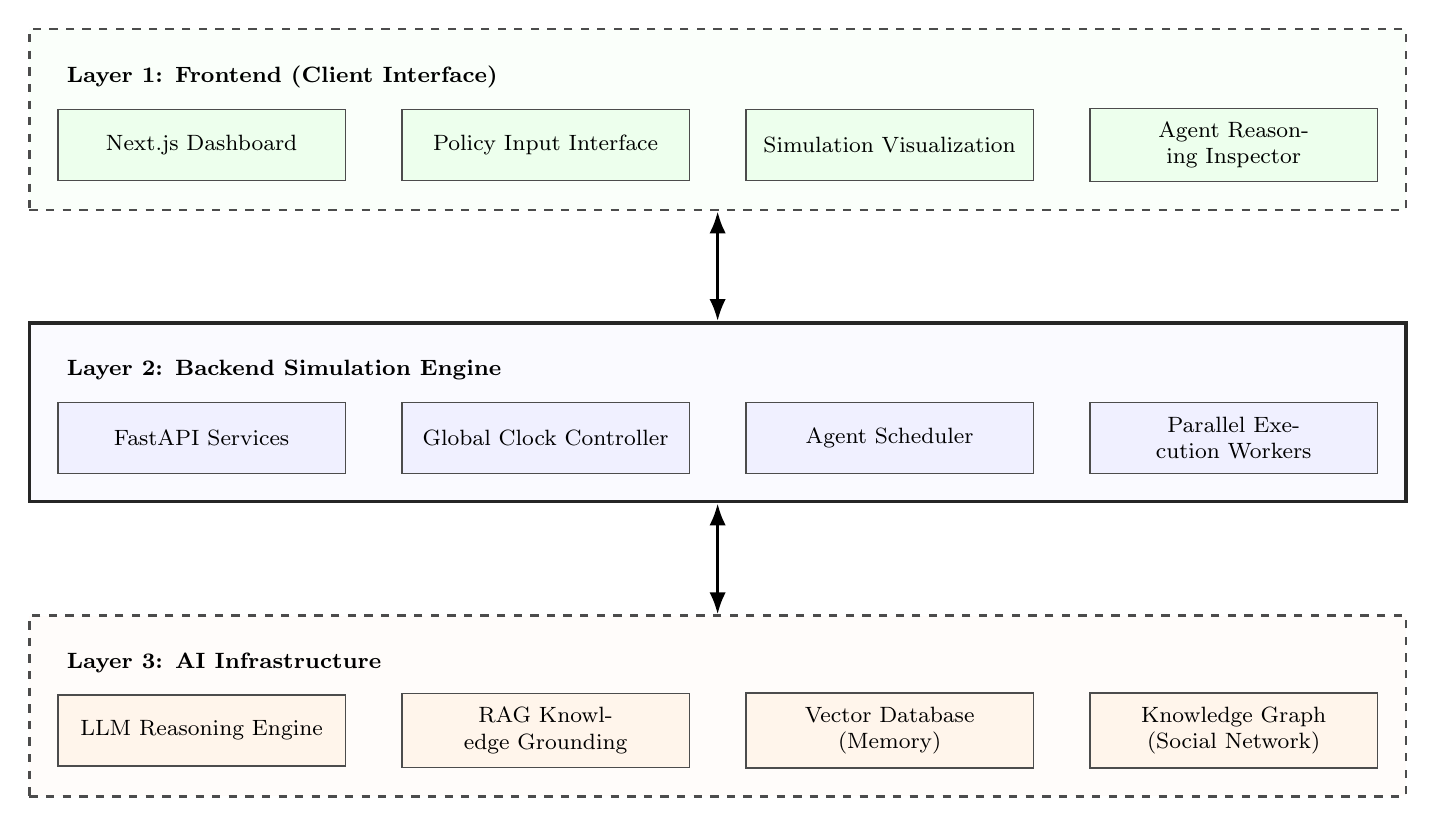
\begin{tikzpicture}[
  font=\footnotesize,
  inode/.style={rectangle, draw=black!70, line width=0.5pt, fill=white, align=center,
                inner sep=5pt, minimum height=9mm, text width=3.3cm, font=\footnotesize},
  dlayer/.style={rectangle, dashed, draw=black!70, line width=0.9pt, inner sep=10pt},
  slayer/.style={rectangle, draw=black!85, line width=1.3pt, inner sep=10pt},
  ltitle/.style={font=\footnotesize\bfseries},
  vv/.style={{Latex[length=2.8mm]}-{Latex[length=2.8mm]}, line width=1.1pt}
]
% ---- Layer 1: Frontend ----
\node[inode, fill=green!7] (f1) {Next.js Dashboard};
\node[inode, fill=green!7, right=7mm of f1] (f2) {Policy Input Interface};
\node[inode, fill=green!7, right=7mm of f2] (f3) {Simulation Visualization};
\node[inode, fill=green!7, right=7mm of f3] (f4) {Agent Reasoning Inspector};
\node[ltitle, above=4mm of f1.north west, anchor=west] (t1) {Layer 1: Frontend (Client Interface)};
\begin{scope}[on background layer]
\node[dlayer, fill=green!2, fit=(t1)(f1)(f2)(f3)(f4)] (L1) {};
\end{scope}
% ---- Layer 2: Backend ----
\node[inode, fill=blue!6, below=28mm of f1] (b1) {FastAPI Services};
\node[inode, fill=blue!6, right=7mm of b1] (b2) {Global Clock Controller};
\node[inode, fill=blue!6, right=7mm of b2] (b3) {Agent Scheduler};
\node[inode, fill=blue!6, right=7mm of b3] (b4) {Parallel Execution Workers};
\node[ltitle, above=4mm of b1.north west, anchor=west] (t2) {Layer 2: Backend Simulation Engine};
\begin{scope}[on background layer]
\node[slayer, fill=blue!2, fit=(t2)(b1)(b2)(b3)(b4)] (L2) {};
\end{scope}
% ---- Layer 3: AI Infrastructure ----
\node[inode, fill=orange!8, below=28mm of b1] (a1) {LLM Reasoning Engine};
\node[inode, fill=orange!8, right=7mm of a1] (a2) {RAG Knowledge Grounding};
\node[inode, fill=orange!8, right=7mm of a2] (a3) {Vector Database (Memory)};
\node[inode, fill=orange!8, right=7mm of a3] (a4) {Knowledge Graph (Social Network)};
\node[ltitle, above=4mm of a1.north west, anchor=west] (t3) {Layer 3: AI Infrastructure};
\begin{scope}[on background layer]
\node[dlayer, fill=orange!2, fit=(t3)(a1)(a2)(a3)(a4)] (L3) {};
\end{scope}
% ---- vertical inter-layer arrows ----
\draw[vv] (L1.south) -- (L2.north);
\draw[vv] (L2.south) -- (L3.north);
\end{tikzpicture}%
}
\caption{PolicySim technical system architecture. The framework is strictly decoupled across a frontend client interface, a high-concurrency backend simulation engine, and a modular AI infrastructure comprising the LLM reasoning engine, retrieval-augmented generation for knowledge grounding, a vector database for agent memory, and a knowledge graph for the social network.}
\label{fig:arch}
\end{figure*}

\section{Hierarchical Cognitive-Social Simulation Architecture}
\label{sec:layers}

Section~\ref{sec:arch} described \emph{how} PolicySim runs, in terms of frontend, backend, and AI infrastructure. This section describes \emph{what} it does, as a stack of six layers that together carry a written policy through to an emergent society and an audited result. The layers mirror the cognitive pipeline introduced earlier: understanding the policy and building the population at the base, individual cognition and social interaction in the middle, world simulation and counterfactual comparison above them, and responsible-AI checks running through the whole stack. Laid out this way, it is clear that PolicySim is not a single model but an architecture in which the language model is only one part.

\subsection{Layer 1: Policy intelligence}
This layer turns natural-language policy into simulation parameters. A \emph{policy parsing agent} reads the document; \emph{regulation extraction} identifies the rules and eligibility conditions; \emph{constraint identification} records the limits the policy imposes (amounts, schedules, and targeting); and a \emph{policy-to-simulation compiler} produces a machine-readable specification that the environment can apply. Because this step is the most error-prone, its output is reviewed and signed off by a human before any run (Section~\ref{sec:resp}).

\subsection{Layer 2: Synthetic society generation}
This layer builds the community. \emph{Demographic sampling} draws an aggregate population that matches public census distributions; \emph{persona generation} expands each sampled record into a coherent individual profile; \emph{behavioral distribution matching} ensures that the spread of attributes and tendencies agrees with known population statistics; and \emph{population calibration} adjusts the result so that summary measures match real data. No synthetic citizen corresponds to a real person: the layer reproduces the \emph{statistical structure} of a community, not its members.

\subsection{Layer 3: Cognitive agent}
Each agent carries an \emph{identity}, a \emph{memory}, a set of \emph{beliefs}, \emph{goals}, \emph{preferences}, and \emph{constraints}, together with a \emph{reasoning engine} (the adapted LLM) and a \emph{decision planner}; the detailed design is given in Section~\ref{sec:agent}. The cognitive core is the way beliefs change over time. We write the belief update of agent $i$ as
\begin{equation}
B_i(t+1) = f\big(B_i(t),\; o_i(t),\; e_i(t)\big),
\end{equation}
where $B_i(t)$ is the agent's current beliefs, $o_i(t)$ is what it observes, $e_i(t)$ is the experience it has just had, and $f$ is the reflection process that combines them. This is how an agent that repeatedly experiences an unreliable service gradually comes to distrust it.

\subsection{Layer 4: Social intelligence}
Agents are connected in a network, and this layer models how they influence one another. It maintains \emph{trust} weights on social ties, governs \emph{information diffusion} along those ties, represents \emph{social influence} on belief and choice, and stores the \emph{community network} itself. The social signal reaching agent $i$ can be written as a trust-weighted combination of its neighbors' states,
\begin{equation}
I_i(t+1) = \sum_{j \in \mathcal{N}(i)} w_{ij}\, B_j(t),
\end{equation}
where $\mathcal{N}(i)$ is the set of neighbors of agent $i$ and $w_{ij}$ is the trust or tie strength from $i$ to $j$. This influence term enters the belief update of Layer~3, so that neighbors shape - but do not dictate - an agent's view. The mechanism lets the same policy spread differently through different parts of a community.

\subsection{Layer 5: Simulation intelligence}
This layer runs the world and supports experimentation. An \emph{environment engine} maintains the shared state and advances it step by step; a \emph{policy intervention engine} applies a compiled policy by changing the rules the agents face; an \emph{emergent behavior detector} aggregates individual actions into population-level patterns; and a \emph{counterfactual scenario generator} makes it possible to ask comparative questions of the form ``what happens if policy A is changed to policy B?'' by running matched simulations that differ only in the policy. Counterfactual comparison is central to policy design, where the question is rarely about one option in isolation but about the difference between alternatives.

\subsection{Layer 6: Responsible AI}
This layer makes the system accountable, and it operates across all the others rather than only at the end. \emph{Bias auditing} screens agent outputs and outcomes for skewed or stereotyped patterns; \emph{uncertainty estimation} quantifies confidence using variation across random seeds and model settings; \emph{explainability} exposes the reasoning behind each result through inspectable agent traces; and \emph{confidence calibration} checks that stated confidence matches observed accuracy. The outputs of this layer are attached to every result, so that no prediction is reported without an accompanying statement of bias, uncertainty, and confidence (Section~\ref{sec:resp}).

\section{Generative Agent Design}
\label{sec:agent}

Each citizen agent is designed to behave like an individual resident (Fig.~\ref{fig:agent}). It has five elements.

\begin{figure}[!t]
\centering
\resizebox{\columnwidth}{!}{%
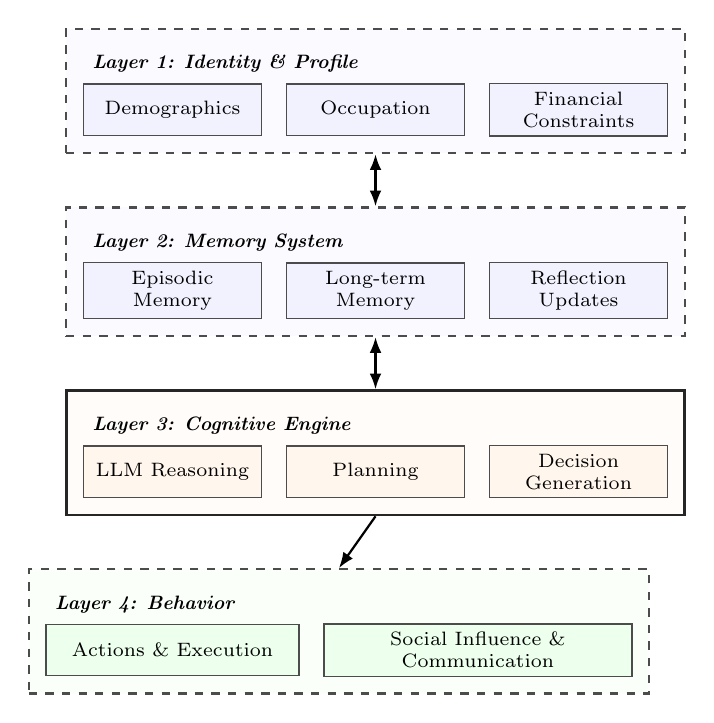
\begin{tikzpicture}[
  font=\scriptsize,
  inode/.style={rectangle, draw=black!70, line width=0.5pt, fill=white, align=center,
                inner sep=3pt, minimum height=6.5mm, text width=2.05cm, font=\scriptsize},
  dlayer/.style={rectangle, dashed, draw=black!70, line width=0.8pt, inner sep=6pt},
  slayer/.style={rectangle, draw=black!85, line width=1pt, inner sep=6pt},
  ltitle/.style={font=\scriptsize\itshape\bfseries},
  vv/.style={{Latex[length=2mm]}-{Latex[length=2mm]}, line width=0.8pt},
  dn/.style={-{Latex[length=2mm]}, line width=0.8pt}
]
% ---- Layer 1: Identity & Profile ----
\node[inode, fill=blue!5] (p1) {Demographics};
\node[inode, fill=blue!5, right=3mm of p1] (p2) {Occupation};
\node[inode, fill=blue!5, right=3mm of p2] (p3) {Financial Constraints};
\node[ltitle, above=2.5mm of p1.north west, anchor=west] (lt1) {Layer 1: Identity \& Profile};
\begin{scope}[on background layer]
\node[dlayer, fill=blue!2, fit=(lt1)(p1)(p2)(p3)] (A1) {};
\end{scope}
% ---- Layer 2: Memory System ----
\node[inode, fill=blue!5, below=16mm of p1] (m1) {Episodic Memory};
\node[inode, fill=blue!5, right=3mm of m1] (m2) {Long-term Memory};
\node[inode, fill=blue!5, right=3mm of m2] (m3) {Reflection Updates};
\node[ltitle, above=2.5mm of m1.north west, anchor=west] (lt2) {Layer 2: Memory System};
\begin{scope}[on background layer]
\node[dlayer, fill=blue!2, fit=(lt2)(m1)(m2)(m3)] (A2) {};
\end{scope}
% ---- Layer 3: Cognitive Engine ----
\node[inode, fill=orange!7, below=16mm of m1] (c1) {LLM Reasoning};
\node[inode, fill=orange!7, right=3mm of c1] (c2) {Planning};
\node[inode, fill=orange!7, right=3mm of c2] (c3) {Decision Generation};
\node[ltitle, above=2.5mm of c1.north west, anchor=west] (lt3) {Layer 3: Cognitive Engine};
\begin{scope}[on background layer]
\node[slayer, fill=orange!2, fit=(lt3)(c1)(c2)(c3)] (A3) {};
\end{scope}
% ---- Layer 4: Behavior ----
\node[inode, fill=green!7, below=16mm of c1, text width=3.0cm] (h1) {Actions \& Execution};
\node[inode, fill=green!7, right=3mm of h1, text width=3.7cm] (h2) {Social Influence \& Communication};
\node[ltitle, above=2.5mm of h1.north west, anchor=west] (lt4) {Layer 4: Behavior};
\begin{scope}[on background layer]
\node[dlayer, fill=green!2, fit=(lt4)(h1)(h2)] (A4) {};
\end{scope}
% ---- arrows ----
\draw[vv] (A1.south) -- (A2.north);
\draw[vv] (A2.south) -- (A3.north);
\draw[dn] (A3.south) -- (A4.north);
\end{tikzpicture}%
}
\caption{Generative citizen agent cognitive architecture. Each agent processes its structural constraints through layered identity, memory, and cognitive components, producing actions and social communication via a continuous loop of observation, memory retrieval, reflection, planning, and action.}
\label{fig:agent}
\end{figure}

\subsection{Profile}
The profile anchors a stable identity: \emph{age}, \emph{occupation}, household, and \emph{socioeconomic context} (income, savings, debts, home and work location, transport access, schedule constraints). Profiles are sampled so that the synthetic population matches the real community's demographics in aggregate (Section~\ref{sec:impl}). Following evidence that rich descriptions yield more accurate and less biased agents than thin demographic labels~\cite{park2024}, each profile is expanded into a short, coherent life narrative rather than a list of attributes.

\subsection{Memory}
Memory gives the agent continuity and learning. \emph{Episodic memory} records specific, time-stamped experiences (``the bus was late and my manager warned me''). \emph{Long-term memory} holds generalizations the agent forms over time (``relying on the bus is risky for my job''). The current situation is used as a query to recall the most relevant memories, combining semantic similarity with how recent and how important each memory is.

\subsection{Goals}
Agents act in pursuit of objectives - paying rent, keeping a job, caring for family - under real constraints. Rather than maximizing a formal utility function, agents \emph{satisfice}: they choose an acceptable option among those that come to mind, which is both more realistic for people under stress and more tractable computationally~\cite{simon1955,mullainathan2013}.

\subsection{Reasoning}
Given its profile, recalled memory, beliefs, and current situation, the agent's LLM generates a behavioral response. The situation is described concretely and with specific numbers and deadlines (for example, an exact cash balance, a rent amount, and a due date), on the hypothesis that such bounded, high-stakes framing elicits the attention-narrowing behavior that the scarcity literature documents~\cite{mullainathan2013}. The LLM produces a brief rationale and then a decision; the decision is constrained to a fixed set of valid actions so that it can be executed and so that impossible actions (spending money one does not have) are rejected.

\subsection{Interaction}
Agents influence each other through the social network. A neighbor's action or message enters one's observation and memory, and the agent weighs it according to how much it trusts the source. What spreads is not a binary ``infected'' flag but a message with content and framing, so the same policy announcement can reassure one person and alarm another. This lets PolicySim represent social contagion and trust dynamics that classical diffusion models cannot~\cite{granovetter1978}.

\section{Multi-Agent Simulation Process}

The simulation advances in discrete time steps (for example, one simulated hour per step). Within a step, all agents act on the same frozen snapshot of the world, and their actions are then reconciled together; this keeps the world causally consistent. \emph{Emergent behavior} - population-level patterns that no single agent's rule dictates - arises from the interaction of many heterogeneous agents over many steps. The lifecycle (Fig.~\ref{fig:agent}) is:

\begin{enumerate}
\item \textbf{Environment creation.} Build the virtual community: the map, institutions, prices, transit, and the policy under test.
\item \textbf{Agent initialization.} Instantiate the population from real demographic data, assign profiles and initial memories, and construct the social network.
\item \textbf{Observation.} Each agent receives a plain-language description of what it can perceive locally (its own situation, local conditions, neighbors' visible actions).
\item \textbf{Memory retrieval.} The agent recalls the most relevant past experiences, scored by similarity, recency, and importance.
\item \textbf{Reflection.} Periodically, the agent distills recent experiences into updated beliefs (for example, growing or losing trust in an institution).
\item \textbf{Planning.} The agent forms or revises a short plan for its day, sequencing intended activities.
\item \textbf{Action generation.} The agent's LLM produces a decision, which is validated against the allowed action set.
\item \textbf{Environment update.} The engine applies all agents' actions together, resolves conflicts (e.g., a balanced financial ledger, limited capacity), updates the world and the social ties, and records each agent's experienced outcome back into memory.
\end{enumerate}
Steps 3--8 repeat each tick; reflection and planning are run periodically rather than every step to control cost.

\section{Technical Implementation}
\label{sec:impl}

PolicySim is designed around mature, open components chosen to fit each task (Table~\ref{tab:stack}).
The \emph{frontend} uses Next.js/React for a responsive console with map and chart visualization.
The \emph{backend} uses FastAPI, a Python web framework whose asynchronous design suits a workload dominated by many concurrent, latency-bound model calls; parallel agent execution is handled by a distributed task queue.
\emph{Data} is stored in three systems because the access patterns genuinely differ: PostgreSQL holds structured world state and the financial ledger, where transactional correctness matters; a vector database (e.g., Chroma) holds episodic memories for similarity search; and a graph database (e.g., Neo4j) holds the social network, where neighbor and path queries are native and efficient. A single relational database with vector and recursive-query extensions is a viable simpler alternative for small populations, and we treat it as a baseline.
For \emph{AI}, citizen agents run a compact open instruction-tuned model (in the 7--8B-parameter class) served by a high-throughput inference engine that uses efficient memory management to keep many agents running concurrently~\cite{kwon2023}; \emph{quantization} (reducing the numerical precision of model weights, e.g., to 4 bits) shrinks each agent's memory footprint so more agents fit on the same hardware, at a small quality cost that we treat as something to measure rather than assume. A larger model is reserved for the infrequent, high-value tasks of policy translation and final reporting. An embedding model converts memories and situations into the vectors used for retrieval.

\begin{table}[!t]
\caption{Technology Choices and Rationale}
\label{tab:stack}
\centering
\renewcommand{\arraystretch}{1.2}
\footnotesize
\begin{tabular}{@{}p{1.5cm}p{2.0cm}p{3.1cm}@{}}
\toprule
\textbf{Layer} & \textbf{Choice} & \textbf{Why} \\
\midrule
Frontend & Next.js / React & Responsive console; map and live-chart visualization; reasoning inspector \\
Backend & FastAPI + task queue & Async I/O fits many concurrent model calls; parallel agent execution \\
State DB & PostgreSQL & Transactions and ledger integrity for world state \\
Memory DB & Vector database & Semantic similarity search over episodic memory \\
Social DB & Graph database & Native neighbor/path queries for social ties and trust \\
Reasoning & Compact open LLM (quantized) + large LLM for system tasks & Throughput and cost for many agents; quality where it matters \\
Grounding & RAG + embedding model & Ground policy translation and retrieval in real text \\
\bottomrule
\end{tabular}
\end{table}

\begin{table}[!t]
\caption{PolicySim AI Architecture Components and Their Roles}
\label{tab:pipeline}
\centering
\renewcommand{\arraystretch}{1.25}
\footnotesize
\begin{tabular}{@{}p{1.45cm}p{1.4cm}p{1.55cm}p{1.7cm}@{}}
\toprule
\textbf{Component} & \textbf{Technology} & \textbf{Purpose} & \textbf{Contribution} \\
\midrule
LLM & Transformer model & Generates agent decisions & Reasoning that interprets context \\
RAG & Retrieval + embeddings & Grounds output in real text & Policy and memory grounding \\
Vector database & Embedding store & Stores agent experience & Continuity and learning over time \\
Knowledge graph & Graph database & Stores social ties & Trust and information diffusion \\
Agent memory & Episodic + long-term & Remembers and reflects & Persona consistency over time \\
Simulation engine & Multi-agent loop & Runs the world forward & Emergent, counterfactual outcomes \\
Responsible AI & Audit + calibration & Checks fairness, uncertainty & Trustworthy, accountable results \\
\bottomrule
\end{tabular}
\end{table}

\section{Real-World Scenario and Human Oversight}
\label{sec:scenario}

To make the framework concrete, this section illustrates how PolicySim would be used on a realistic municipal scenario and how a human policymaker stays in control of the process.

\subsection{A community simulation scenario}
Consider a city department evaluating a transit-subsidy program. The relevant community is more than a list of individuals: it includes residents, a transportation network, healthcare and housing systems, and the nonprofit organizations that deliver services. PolicySim represents these as a digital twin (Fig.~\ref{fig:scenario}). A real policy is translated into the twin, the simulation is run forward, and the framework reports the predicted community outcomes - who gains access, how travel and appointment-keeping change, and which groups are missed. Because the twin is built only from public, aggregated data, it models the structure of the community rather than any real person.

\begin{figure*}[!t]
\centering
\resizebox{\textwidth}{!}{%
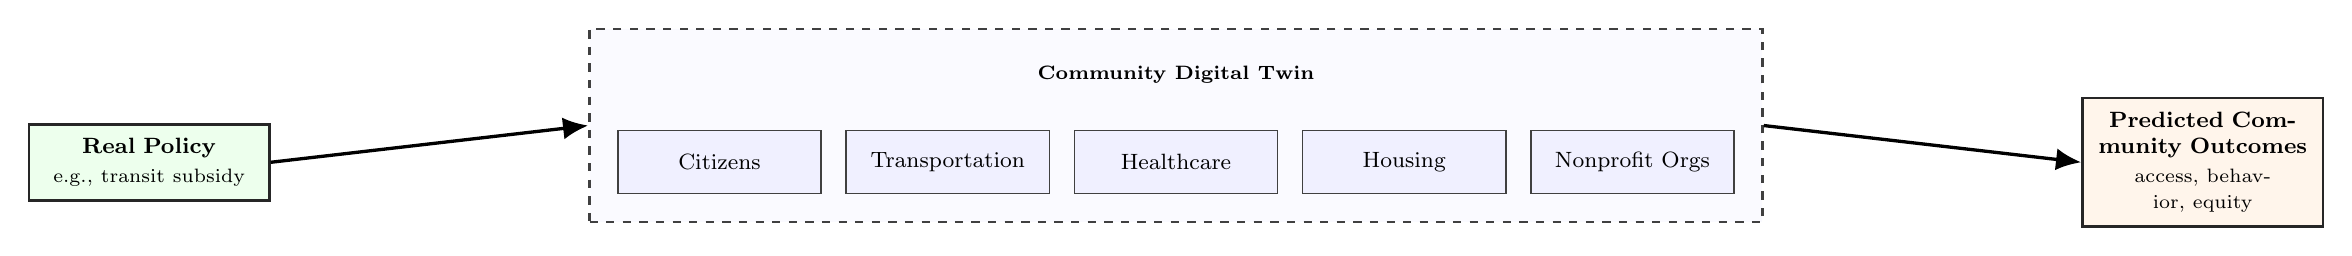
\begin{tikzpicture}[
  font=\footnotesize,
  inode/.style={rectangle, draw=black!75, line width=0.5pt, fill=white, align=center,
                inner sep=4pt, minimum height=8mm, text width=2.3cm, font=\footnotesize},
  bignode/.style={rectangle, draw=black!85, line width=1pt, fill=white, align=center,
                  inner sep=5pt, minimum height=9mm, text width=2.7cm, font=\footnotesize},
  dpanel/.style={rectangle, draw=black!75, dashed, line width=0.9pt, inner sep=10pt},
  ptitle/.style={font=\scriptsize\bfseries},
  bigar/.style={-{Latex[length=3.2mm,width=2.8mm]}, line width=1.2pt}
]
\node[bignode, fill=green!7] (pol) {\textbf{Real Policy}\\[1pt]{\scriptsize e.g., transit subsidy}};
\node[inode, fill=blue!6, right=44mm of pol] (cz) {Citizens};
\node[inode, fill=blue!6, right=3mm of cz] (tr) {Transportation};
\node[inode, fill=blue!6, right=3mm of tr] (hc) {Healthcare};
\node[inode, fill=blue!6, right=3mm of hc] (ho) {Housing};
\node[inode, fill=blue!6, right=3mm of ho] (np) {Nonprofit Orgs};
\node[ptitle] (tw) at ([yshift=7mm]$(cz.north)!0.5!(np.north)$) {Community Digital Twin};
\begin{scope}[on background layer]
\node[dpanel, fill=blue!2, fit=(cz)(tr)(hc)(ho)(np)(tw)] (twin) {};
\end{scope}
\node[bignode, fill=orange!8, right=44mm of np] (out) {\textbf{Predicted Community Outcomes}\\[1pt]{\scriptsize access, behavior, equity}};
\draw[bigar] (pol.east) -- (twin.west);
\draw[bigar] (twin.east) -- (out.west);
\end{tikzpicture}%
}
\caption{Real-world policy simulation scenario. A real policy is translated into a community digital twin - residents, transportation, healthcare, housing, and the nonprofit organizations that deliver services - and the simulation reports the predicted community outcomes. The twin is built only from public, aggregated data.}
\label{fig:scenario}
\end{figure*}

\subsection{Human-in-the-loop decision process}
PolicySim is designed to inform a decision, not to make one. Figure~\ref{fig:hitl} shows the intended workflow. A policymaker poses a question and a candidate policy; PolicySim runs the simulation and produces recommendations together with predicted outcomes; a risk-and-fairness analysis is attached, stating where the result is uncertain and which groups may be affected unevenly; and the policymaker, seeing both the prediction and its limits, makes the final decision and may revise the policy and repeat. The human reviews the translated policy before any run and the evidence after it, so accountability stays with the institution throughout.

\begin{figure}[!t]
\centering
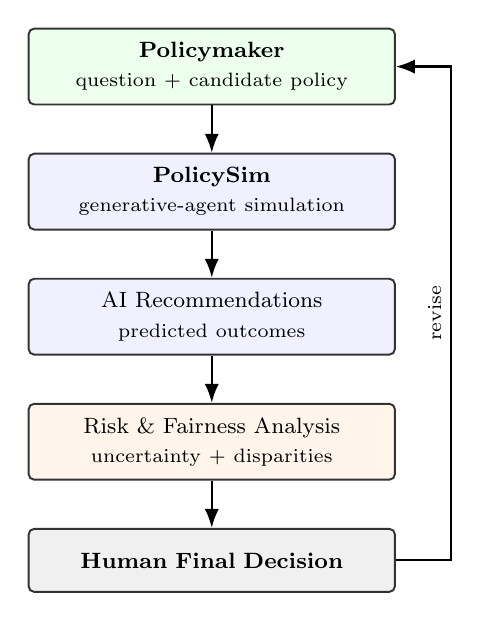
\begin{tikzpicture}[
  font=\footnotesize, node distance=6mm,
  pbox/.style={rectangle, rounded corners=2pt, draw=black!80, line width=0.7pt, fill=white,
               align=center, inner sep=5pt, minimum height=8mm, text width=4.3cm, font=\footnotesize},
  dn/.style={-{Latex[length=2.4mm]}, line width=0.8pt}
]
\node[pbox, fill=green!7] (a) {\textbf{Policymaker}\\[1pt]{\scriptsize question + candidate policy}};
\node[pbox, fill=blue!6, below=of a] (b) {\textbf{PolicySim}\\[1pt]{\scriptsize generative-agent simulation}};
\node[pbox, fill=blue!6, below=of b] (c) {AI Recommendations\\[1pt]{\scriptsize predicted outcomes}};
\node[pbox, fill=orange!8, below=of c] (d) {Risk \& Fairness Analysis\\[1pt]{\scriptsize uncertainty + disparities}};
\node[pbox, fill=gray!12, below=of d] (e) {\textbf{Human Final Decision}};
\draw[dn] (a) -- (b);
\draw[dn] (b) -- (c);
\draw[dn] (c) -- (d);
\draw[dn] (d) -- (e);
\draw[dn] (e.east) -- ++(0.7,0) |- (a.east);
\node[font=\scriptsize, anchor=south, rotate=90] at ([xshift=0.7cm]$(a.east)!0.5!(e.east)$) {revise};
\end{tikzpicture}
\caption{PolicySim human-in-the-loop decision process. The policymaker supplies a question and a candidate policy; PolicySim returns recommendations and predicted outcomes; a risk-and-fairness analysis states the limits of the result; and the human makes the final decision, optionally revising the policy and repeating. Accountability remains with the human throughout.}
\label{fig:hitl}
\end{figure}

\section{Evaluation Methodology}
\label{sec:eval}

Everything in PolicySim depends on one question: does its synthetic behavior match how people really act? Evaluation is therefore the core of the work, not a closing formality, and it cannot rest on accuracy alone. A simulation can reproduce an aggregate number while the behavior beneath it is implausible, and it can generate convincing individuals whose collective outcome is still wrong. To guard against both failures, we assess PolicySim along seven dimensions, moving from predictive accuracy, through the realism of individual agents and of the society they form, to fairness, self-knowledge, and cost. Each dimension answers a specific question, and Table~\ref{tab:eval} gathers the complete set. The scores introduced below are \emph{proposed} instruments: their component weights would be fixed and reported for a given study rather than assumed, and the experiments of Section~\ref{sec:expdesign} are what would put them to use.

Our main testbed is \emph{historical backtesting}, which runs the simulation against the past. We build the virtual community from a baseline year, introduce a real policy that was enacted at that time, and simulate forward using only information available at the start, then compare the simulated outcomes with what was actually recorded. A simulation that recovers the real change more accurately than a calibrated classical baseline has shown predictive, not merely plausible, fidelity. The main threat is that the model may already ``know'' what happened after the baseline year from its training data; we limit this by favoring local, less-documented outcomes and by checking the model for such leakage, and we treat any contaminated case as exploratory rather than confirmatory.

\begin{table*}[!t]
\caption{The PolicySim Evaluation Framework}
\label{tab:eval}
\centering
\renewcommand{\arraystretch}{1.3}
\footnotesize
\begin{tabular}{@{}p{2.5cm}p{4.0cm}p{4.0cm}p{4.6cm}@{}}
\toprule
\textbf{Dimension} & \textbf{Metric(s)} & \textbf{Purpose} & \textbf{Research question} \\
\midrule
Predictive accuracy & MAE, RMSE, MAPE, directional accuracy & Match recorded outcomes & How close are predictions to reality? \\
Behavioral realism & ABFS, APCS & Lifelike individual agents & Do agents behave like real people? \\
Social simulation quality & SEAS, network similarity (degree, clustering, community) & Realistic collective behavior & Does a believable community emerge? \\
Policy decision & CPRA & Compare policy options & Can it rank policy A against B correctly? \\
Responsible AI & Demographic parity, disparate-impact ratio, BAS & Fair and non-distorting results & Can the output be trusted to be fair? \\
Uncertainty and reliability & Expected calibration error, seed variance & Honest confidence and stability & Does the system know its own limits? \\
Computational performance & Runtime, tokens per agent, memory, scaling & Affordable at community scale & Can a small organization run it? \\
\bottomrule
\end{tabular}
\end{table*}

\subsection{Predictive accuracy}
The first question is the most direct: how close are the simulated outcomes to the real ones? For a scalar outcome such as a take-up rate or a transit share, we report the mean absolute error and the root mean square error,
\begin{equation}
\mathrm{MAE} = \frac{1}{n}\sum_{i=1}^{n}\lvert y_i - \hat{y}_i\rvert, \quad
\mathrm{RMSE} = \sqrt{\frac{1}{n}\sum_{i=1}^{n}(y_i - \hat{y}_i)^2},
\end{equation}
where $y_i$ is the recorded value and $\hat{y}_i$ the simulated one; RMSE weighs large misses more heavily than MAE. Because policies differ widely in scale, an absolute error is hard to compare across outcomes, so we also report the mean absolute percentage error,
\begin{equation}
\mathrm{MAPE} = \frac{100}{n}\sum_{i=1}^{n}\left\lvert \frac{y_i - \hat{y}_i}{y_i}\right\rvert,
\end{equation}
which states the error as a share of the true value. Relative error matters in policy work because the same absolute gap can be trivial for one outcome and decisive for another, and MAPE makes a five-point miss on a small program comparable to one on a large program. We add \emph{directional accuracy}, the fraction of cases in which the simulation gets the \emph{sign} of the change right, since a decision often turns first on whether a policy raises or lowers access and only later on the exact figure. Where an outcome is a whole distribution rather than a single number, such as the spread of income, we compare the simulated and real distributions with the Jensen--Shannon divergence and the Wasserstein distance, which measure how far apart two distributions lie.

\subsection{Agent behavioral realism}
Accuracy at the aggregate says nothing about whether the individual agents behave like real people, so the second dimension looks inside the simulation. Realism has several faces that no single distance captures, so we summarize them with a proposed \emph{Agent Behavioral Fidelity Score},
\begin{equation}
\mathrm{ABFS} = \alpha B + \beta S + \gamma M + \delta I, \qquad \alpha + \beta + \gamma + \delta = 1,
\end{equation}
where $B$ is how closely agent behavior matches documented real-world patterns, $S$ is how closely the structure of social interaction matches, $M$ is how consistent an agent stays with its own memory and persona over time, and $I$ is the realism of individual decisions. The weights are chosen and reported per study, and the score is meant to make these aspects explicit rather than to replace the individual measures. A closely related concern is whether an agent stays in character, since real people are reasonably consistent: their choices line up with their circumstances and their history. We capture this with a proposed \emph{Agent Persona Consistency Score},
\begin{equation}
\mathrm{APCS} = \lambda_1 P + \lambda_2 M + \lambda_3 D, \qquad \lambda_1 + \lambda_2 + \lambda_3 = 1,
\end{equation}
where $P$ measures agreement between an agent's actions and its stated background, goals, and financial constraints, $M$ measures agreement with its own earlier experiences, and $D$ measures whether successive decisions remain coherent rather than drifting at random. A low APCS is an early warning that the model is losing the thread of the character it is meant to play.

\subsection{Social simulation quality}
Realistic individuals are necessary but not sufficient; the point of PolicySim is the society that forms when they interact. The third dimension asks whether community-level behavior is realistic. We track how individual choices turn into collective outcomes, for example how a subsidy is taken up over time, how trust in an agency rises or falls, and how information moves through the network, and we summarize the agreement between these simulated trajectories and the real ones in a proposed \emph{Social Emergence Accuracy Score}. In practice this compares simulated and observed curves for adoption, trust, and information spread, so that a model which produces plausible individuals but the wrong diffusion pattern is still marked down. The network itself must also be realistic, because diffusion depends on its shape. We therefore compare the simulated community network with the real one on three properties: the similarity of their degree distributions (how many ties people have), the similarity of their clustering (how often a person's contacts are also connected to each other), and the similarity of their community structure (whether the same kinds of dense groups appear). A network that matches on these properties is far more likely to reproduce real patterns of contagion and influence.

\subsection{Policy decision evaluation}
A policymaker rarely needs the exact value of a single outcome; more often they need to know which of two options is better. The fourth dimension measures this directly through \emph{Counterfactual Policy Ranking Accuracy}, the share of paired comparisons in which the simulation orders two policies the way reality does, $\mathrm{CPRA} = (\text{correct rankings})/(\text{total comparisons})$. Ranking is a more forgiving and often more useful target than absolute prediction: a model whose levels are biased can still place options in the right order, and the right order is usually what a decision requires. A high CPRA therefore means PolicySim is a useful comparator even where its point predictions are imperfect.

\subsection{Responsible-AI evaluation}
A simulation of vulnerable people can be accurate on average and still be untrustworthy if it treats some groups unfairly or distorts the differences between them. The fifth dimension checks this. We measure fairness with demographic parity, which asks whether the rate of receiving a benefit is similar across groups, and with the disparate-impact ratio, the ratio of those rates between two groups, where a value far from one signals unequal treatment. Beyond static fairness, we ask whether the simulation \emph{amplifies} existing inequality, a documented failure mode of LLM-based social models~\cite{bisbee2024,santurkar2023}. A proposed \emph{Bias Amplification Score}, $\mathrm{BAS} = (\text{simulated disparity})/(\text{real disparity})$, makes this visible: a value above one means the model exaggerates a real gap, a value below one means it hides part of it, and a value near one means it neither invents nor erases inequality. Catching amplification matters more here than almost anywhere else, since an exaggerated disparity could be used to justify a harmful decision.

\subsection{Uncertainty and reliability}
A trustworthy system should know when it is unsure. The sixth dimension measures whether PolicySim's confidence is honest and whether its results are stable. \emph{Calibration} asks whether stated confidence matches observed accuracy: predictions made with eighty-percent confidence should be correct about eighty percent of the time. We quantify this with the expected calibration error,
\begin{equation}
\mathrm{ECE} = \sum_{m=1}^{M} \frac{\lvert B_m\rvert}{n}\,\bigl\lvert \mathrm{acc}(B_m) - \mathrm{conf}(B_m)\bigr\rvert,
\end{equation}
which sorts predictions into $M$ confidence bins $B_m$, compares the average accuracy and the average confidence within each bin, and averages the gaps in proportion to how many predictions fall in each bin; a small ECE means the confidence can be believed. Because agent decisions are stochastic, we also check \emph{stability} by running the same scenario under many random seeds and measuring how far the key outputs move, using the variance $\sigma^2 = \tfrac{1}{n}\sum_i (x_i - \mu)^2$ around their mean $\mu$. Low variance means the conclusions are reproducible rather than artifacts of one random draw, and every headline result is reported with an interval rather than as a single point.

\subsection{Computational performance}
The last dimension is practical. PolicySim is meant for nonprofits and community organizations, so cost decides whether it can be used at all. We measure runtime, the number of tokens consumed per agent per step, and peak memory, and we study how these grow as the population scales from roughly one hundred to one thousand to ten thousand agents. Reporting cost next to accuracy keeps the trade-off honest: a more faithful configuration is only useful if a small organization can actually afford to run it.

\subsection{From many scores to one judgment}
Taken together, these seven dimensions describe a simulation that is accurate, behaviorally and socially realistic, fair, honest about its uncertainty, and affordable. For a single reporting figure, the dimension scores can be combined into one overall \emph{Simulation Reality Alignment Score}, with the weights fixed and disclosed in advance. We prefer, however, to keep the individual scores in view, because a strong average can hide a serious weakness in one dimension, and in public-interest work that hidden weakness is usually the one that matters most. This is the deeper reason a social simulation cannot be judged by accuracy alone: a model can predict the right numbers while misrepresenting people, distorting inequality, or overstating its own confidence, and only a spread of metrics like this one can tell the difference.

\section{Responsible AI Considerations}
\label{sec:resp}

PolicySim models how vulnerable people respond to policy, so responsible design is a requirement, not an addendum.

\textbf{Bias.} LLMs inherit biases from their training data, and careless prompting can produce caricatures of groups rather than faithful representations. We mitigate this by conditioning on rich personal narratives rather than thin labels (which reduces cross-group error~\cite{park2024}), by auditing outcomes for disparities, and by measuring amplification and variance collapse directly. Bias is \emph{measured and reported per group}, never assumed absent.

\textbf{Hallucination.} LLMs can produce fluent but unfounded statements. We reduce this risk structurally: agents may only emit actions from a validated set, the reporting agent may summarize only computed results, and every claim in a report links back to the underlying metric or agent trace.

\textbf{Privacy.} PolicySim uses only anonymized public data (such as census microdata samples) and synthetic profiles. No agent corresponds to a real person; the virtual community is a model of a population's \emph{statistical and structural} properties, not of any individual. The system stores no personally identifiable information.

\textbf{Transparency.} Results are presented with their uncertainty and with an explicit \emph{validity estimate} - a summary of how far the simulation can be trusted for the specific policy and outcome - and users can inspect the agent reasoning behind any result.

\textbf{Trust calibration engine.} These ideas are brought together in a \emph{trust calibration engine} that accompanies every prediction with three quantities: a \emph{confidence} level (how sure the system is), a \emph{reliability} estimate (how accurate the system has been on similar questions during validation), and a \emph{bias} estimate (whether the result may favor or disadvantage particular groups). Reporting these together turns each output into a claim the user can weigh rather than a number to be taken on faith. The engine is the operational form of the responsible-AI layer of Section~\ref{sec:layers}, and its calibration is measured directly (Section~\ref{sec:eval}).

\textbf{Human oversight.} PolicySim is decision support, not automated policymaking. Translating a policy into simulation parameters requires human review and sign-off; results are advisory and carry their limitations explicitly. This stance is principled, not merely cautious: the system's outputs are estimates from a model of contested fidelity, and allocating public resources is an act of legitimate authority that belongs to accountable human institutions, not to a simulation. A particular hazard is \emph{automation bias} - a polished, confident system can induce over-reliance, especially where it is least reliable. The framework is therefore designed to \emph{calibrate} trust by foregrounding uncertainty and reliability, and whether this design works is itself a research question (Section~\ref{sec:expdesign}).

\section{Experimental Design}
\label{sec:expdesign}

We propose the following experiments, each stated with its expected outcome and the conditions under which the expectation would fail. Experiments~1--3 compare PolicySim with external baselines and probe agent realism; Experiments~4--6 are internal ablations that isolate the contribution of adaptation, memory, and social structure.

\textbf{Experiment~1: Generative agents vs.\ classical ABM.}
On identical scenarios and outcomes, compare PolicySim against a classical rule-based ABM (and against econometric and survey-extrapolation baselines) using the metrics of Section~\ref{sec:eval}.
\emph{Hypothesis.} PolicySim more accurately reproduces outcomes driven by reasoning and communication - especially benefit take-up under procedural friction and the resulting distributional shifts - while classical models may remain competitive on purely mechanical outcomes.
\emph{Expected result.} A measured advantage for PolicySim on cognition-driven outcomes; if no advantage appears, that bounds the value of generative agents for this task and is reported as such.

\textbf{Experiment~2: Agent behavioral realism.}
Assess whether individual agents behave like real people: do they reproduce known behavioral regularities, and can expert raters distinguish simulated from real (anonymized) behavior above chance?
\emph{Hypothesis.} Agents grounded in rich profiles will match documented regularities within published bounds and will be difficult to distinguish from real behavior on the dimensions tested.
\emph{Expected result.} High behavioral plausibility on common situations, with degradation on populations under-represented in the model's training data - an important boundary to characterize.

\textbf{Experiment~3: Policy prediction quality.}
Run the historical-backtesting protocol over several real interventions and policy classes, measuring how accurately PolicySim forecasts recorded outcomes, and producing a per-domain map of where it is and is not trustworthy.
\emph{Hypothesis.} Accuracy will be acceptable for some policy classes (e.g., assistance take-up) and weaker for others; reliability will vary by outcome and group.
\emph{Expected result.} A calibrated ``trust map'' - the practical deliverable - rather than a single headline accuracy number.

\textbf{Experiment~4: Base agents vs.\ adapted and aligned agents.}
Compare citizen agents that use the base foundation model directly against agents adapted and aligned with the pipeline of Sections~\ref{sec:adapt} and~\ref{sec:align} (domain fine-tuning, retrieval grounding, and constraint enforcement).
\emph{Hypothesis.} Adaptation and grounding improve behavioral fidelity (ABFS) and reduce infeasible or off-persona actions, while leaving behavioral diversity intact.
\emph{Expected result.} Higher fidelity and fewer constraint violations for the adapted agents; if alignment is applied too aggressively, we expect a measurable drop in behavioral diversity, which we monitor as a warning sign.

\textbf{Experiment~5: Effect of memory.}
Compare agents with the full memory system against agents whose episodic and long-term memory are disabled.
\emph{Hypothesis.} Memory improves the consistency of agents over time and the realism of adaptation (for example, learning to distrust an unreliable service), raising the memory-consistency and behavioral components of ABFS.
\emph{Expected result.} More coherent long-run behavior with memory; without it, agents should appear forgetful and less realistic, especially over long simulations.

\textbf{Experiment~6: Effect of the social network.}
Compare a full simulation against one in which agents are isolated, with no social ties or information propagation.
\emph{Hypothesis.} The social network is necessary to reproduce diffusion effects - how information and trust spread - so disabling it should change population-level outcomes such as adoption curves.
\emph{Expected result.} Isolated agents should miss contagion dynamics and therefore under- or over-estimate uptake relative to the networked simulation and to real data; the size of this gap measures how much social structure matters for a given policy.

\textbf{Experiment~7: Counterfactual policy testing.}
Run matched simulations that differ only in the policy - an original policy A and an alternative policy B - and measure the difference in outcomes.
\emph{Hypothesis.} PolicySim produces consistent, interpretable differences between policy variants, so that the \emph{relative} ranking of options is stable even where absolute predictions are uncertain.
\emph{Expected result.} Reliable directional and ranking information across variants; this comparative use is often more decision-relevant, and more defensible, than any single absolute forecast.

\textbf{Experiment~8: Agent scaling study.}
Run the same scenario with populations of roughly $10^2$, $10^3$, and $10^4$ agents, and measure accuracy, computational cost, and the strength of emergent effects.
\emph{Hypothesis.} Accuracy and emergent structure improve with scale up to a point, after which cost grows faster than benefit.
\emph{Expected result.} A characterization of the accuracy--cost trade-off and of the scale at which key emergent behaviors, such as diffusion cascades, appear; this informs how large a simulation a given question actually requires.

\textbf{Experiment~9: Graded memory ablation.}
Extending Experiment~5, compare three settings - no memory, short-term memory only, and full long-term memory with reflection - to isolate how much each level of memory contributes.
\emph{Hypothesis.} Realism and consistency increase with memory depth, with the largest gain from adding long-term memory and reflection.
\emph{Expected result.} A graded improvement in the memory-consistency and behavioral components of ABFS as memory deepens, clarifying which aspects of behavior require long-term memory rather than short-term context alone.

\textbf{Experiment~10: Responsible-AI layer ablation.}
Run the system with and without the responsible-AI layer, removing in turn the fairness auditing, the calibration of uncertainty, and the human-review step, and measure how far trust in the output degrades.
\emph{Hypothesis.} Each component contributes to warranted trust, so removing one should make the system either less fair, less honest about its uncertainty, or less accountable, in ways the fairness and calibration metrics can detect.
\emph{Expected result.} A measurable rise in calibration error and in unreported disparity once the layer is removed, which would show that the responsible-AI components do real work rather than serving as decoration.

A planned human-centered study complements these: policymakers complete decision tasks with and without PolicySim, and with and without the validity estimates and reasoning traces, to test whether the design calibrates trust and reduces automation bias.

\section{Discussion}

\textbf{Not just a chatbot.} Because several familiar tools also use language models, it helps to say plainly how PolicySim differs from them. A conversational assistant such as ChatGPT handles one exchange at a time, with no memory carried from session to session. A retrieval-augmented system adds grounding in documents, but it still returns an answer rather than a society. A traditional ABM simulates many interacting agents, yet its agents follow fixed rules and cannot read language. A prediction model maps inputs to an outcome without showing how that outcome comes about. PolicySim is different in kind: it sustains a standing population of agents, each with its own memory, that act and react over time so that population-level behavior emerges from their interaction. The language model is one part of the machine, not the whole of it; the contribution is the surrounding architecture that supplies memory, social structure, a simulated world, counterfactual comparison, and responsible-AI checking. Put simply, PolicySim shifts the use of AI from generating an answer toward simulating a social process, and what it returns is not a reply but a spread of possible community outcomes, each carrying an estimate of how far it can be trusted.

\textbf{Strengths.} The framework's central advantage is that its agents reason over qualitative, language-based situations, the confusing forms, mixed signals, and social pressures that rule-based models cannot express. This makes it possible to treat trust, misunderstanding, and the spread of information as first-class phenomena, and it makes scenario testing cheap, since many variants of a policy can be explored without putting anyone at risk.

\textbf{Limitations.} The most serious limitation is the gap between the simulation and reality. An LLM is a model of text about behavior, and nothing guarantees that this carries over to how people actually act under a new policy. The evidence points both ways, encouraging on survey replication~\cite{argyle2023,park2024} and discouraging on polarization and well-being~\cite{bisbee2024,pataranutaporn2025}, and which way it points for a particular policy is exactly what our evaluation is meant to find out. Cost is a second concern: large runs need substantial computing power, which could confine the tool to well-funded organizations, an equity-of-access worry we take seriously. Finally, the known weaknesses of LLMs, including bias, fabrication, and sensitivity to how a prompt is phrased, mean that results must come with uncertainty and robustness checks, and that conclusions should be read at the level of the population, which we expect to be steadier, rather than from any single agent's path.

\textbf{Bias and over-reliance.} Two risks deserve separate mention. Because agents inherit the biases in their training data, the simulation may portray some groups less faithfully than others, which is why we measure bias and per-group fidelity rather than assume they are fine, and why we prefer rich personal descriptions to thin labels. And because a confident, fluent system invites over-reliance, a busy official may take a prediction as fact, most dangerously for the under-served groups where the model is weakest. PolicySim answers this by attaching uncertainty and fairness information to every result and by keeping a person in the loop, but the risk is real and is itself a subject for study (Section~\ref{sec:expdesign}).

\textbf{In sum.} Taken together, these points define a modest but useful role. PolicySim is not an oracle to be trusted blindly; it is an instrument for making the likely human consequences of a policy visible and open to argument before the policy is enacted. Its value rises as its fidelity is measured honestly, its uncertainty is reported plainly, and its use stays under human control.

\section{Future Work}

Several directions extend the framework. \emph{Real-time community digital twins} would update the simulation continuously from live public data, supporting situational awareness during an active program rather than only retrospective study. \emph{Multimodal and vision-language agents} would let agents perceive non-text signals - maps, forms, and images - so that, for example, the visual difficulty of an application becomes representable. \emph{Reinforcement-learning calibration} against real behavioral traces could make agents not only plausible but \emph{fit} to observed behavior, while guarding against overfitting that would erase the general reasoning that motivates generative agents. \emph{Self-improving agents} could identify where their own fidelity is weakest and request the data that would most reduce their uncertainty. Finally, \emph{federated community models} would let several organizations improve shared agent models without pooling sensitive local data, by exchanging model updates rather than records. Across all of these, the guiding constraint remains that fidelity must be measurable, uncertainty honest, and human judgment central.

\section{Conclusion}

PolicySim argues for a change in what we ask computational tools to do in policy work: to move from \emph{predicting outcomes} toward \emph{simulating the human reasoning and social interaction that produce those outcomes}. Cast as a trustworthy generative social digital twin, it treats a community not as a system of equations but as a population of agents who reason, remember, and are connected to one another, and whose interactions generate the outcomes a policymaker cares about. By placing Large Language Models inside those agents, it can represent the soft frictions, misunderstanding, distrust, and social contagion, that decide whether a policy succeeds and that rule-based and aggregate models cannot reach.

The work can be summarized as four contributions: a generative-agent architecture for policy simulation; a cognitive and social digital-twin design that models people, institutions, infrastructure, and relationships together; a responsible-AI framework for trustworthy decision support, complete with a trust-calibration mechanism and fidelity metrics; and an evaluation-first methodology built on historical backtesting and the honest reporting of uncertainty. At every step we have tried to keep separate what is proposed, what is hypothesized, and what must still be validated, and to keep the documented failure modes of LLM-based simulation in plain sight rather than out of view.

The deeper motivation is public benefit. If the approach proves faithful enough for even some classes of policy, it offers small and stretched organizations a safe way to see friction and unequal impact coming before real people are affected; if it does not, the same methodology still helps, by setting limits on the claims of a fast-moving technology and shielding communities from misplaced trust. Responsible AI and human-centered support are therefore not features added at the end but commitments built in from the start. PolicySim is not meant to replace policymakers; it offers them a controlled setting in which to explore what a policy might do before its effects reach a real community. More broadly, we believe the next generation of AI systems should aim not only to answer questions but to help people understand complex social outcomes, and to do so responsibly.

\begin{thebibliography}{00}

\bibitem{park2023} J. S. Park, J. C. O'Brien, C. J. Cai, M. R. Morris, P. Liang, and M. S. Bernstein, ``Generative agents: Interactive simulacra of human behavior,'' in \emph{Proc. 36th Annu. ACM Symp. User Interface Softw. Technol. (UIST)}, 2023, pp.\ 1--22.

\bibitem{park2024} J. S. Park, C. Q. Zou, A. Shaw, B. M. Hill, C. Cai, M. R. Morris, R. Willer, P. Liang, and M. S. Bernstein, ``Generative agent simulations of 1,000 people,'' arXiv:2411.10109, 2024.

\bibitem{argyle2023} L. P. Argyle, E. C. Busby, N. Fulda, J. R. Gubler, C. Rytting, and D. Wingate, ``Out of one, many: Using language models to simulate human samples,'' \emph{Political Analysis}, vol.\ 31, no.\ 3, pp.\ 337--351, 2023.

\bibitem{bisbee2024} J. Bisbee, J. D. Clinton, C. Dorff, B. Kenkel, and J. M. Larson, ``Synthetic replacements for human survey data? The perils of large language models,'' \emph{Political Analysis}, vol.\ 32, no.\ 4, pp.\ 401--416, 2024.

\bibitem{pataranutaporn2025} P. Pataranutaporn, N. Powdthavee, C. Archiwaranguprok, and P. Maes, ``Simulating human well-being with large language models: Systematic validation and misestimation across 64,000 individuals from 64 countries,'' \emph{Proc. Nat. Acad. Sci.}, vol.\ 122, no.\ 48, e2519394122, 2025.

\bibitem{vezhnevets2023} A. S. Vezhnevets \emph{et al.}, ``Generative agent-based modeling with actions grounded in physical, social, or digital space using Concordia,'' arXiv:2312.03664, 2023.

\bibitem{piao2025} J. Piao \emph{et al.}, ``AgentSociety: Large-scale simulation of LLM-driven generative agents advances understanding of human behaviors and society,'' arXiv:2502.08691, 2025.

\bibitem{gao2024} C. Gao, X. Lan, N. Li, Y. Yuan, J. Ding, Z. Zhou, F. Xu, and Y. Li, ``Large language models empowered agent-based modeling and simulation: A survey and perspectives,'' \emph{Humanit. Soc. Sci. Commun.}, vol.\ 11, no.\ 1, 2024.

\bibitem{schelling1971} T. C. Schelling, ``Dynamic models of segregation,'' \emph{J. Math. Sociol.}, vol.\ 1, no.\ 2, pp.\ 143--186, 1971.

\bibitem{epstein1996} J. M. Epstein and R. Axtell, \emph{Growing Artificial Societies: Social Science from the Bottom Up}. Washington, DC, USA: Brookings Inst. Press / MIT Press, 1996.

\bibitem{simon1955} H. A. Simon, ``A behavioral model of rational choice,'' \emph{Quart. J. Econ.}, vol.\ 69, no.\ 1, pp.\ 99--118, 1955.

\bibitem{mullainathan2013} S. Mullainathan and E. Shafir, \emph{Scarcity: Why Having Too Little Means So Much}. New York, NY, USA: Times Books, 2013.

\bibitem{granovetter1978} M. Granovetter, ``Threshold models of collective behavior,'' \emph{Amer. J. Sociol.}, vol.\ 83, no.\ 6, pp.\ 1420--1443, 1978.

\bibitem{wei2022} J. Wei \emph{et al.}, ``Chain-of-thought prompting elicits reasoning in large language models,'' in \emph{Adv. Neural Inf. Process. Syst. (NeurIPS)}, 2022.

\bibitem{yao2023} S. Yao, J. Zhao, D. Yu, N. Du, I. Shafran, K. Narasimhan, and Y. Cao, ``ReAct: Synergizing reasoning and acting in language models,'' in \emph{Proc. Int. Conf. Learn. Represent. (ICLR)}, 2023.

\bibitem{shinn2023} N. Shinn, F. Cassano, A. Gopinath, K. Narasimhan, and S. Yao, ``Reflexion: Language agents with verbal reinforcement learning,'' in \emph{Adv. Neural Inf. Process. Syst. (NeurIPS)}, 2023.

\bibitem{santurkar2023} S. Santurkar, E. Durmus, F. Ladhak, C. Lee, P. Liang, and T. Hashimoto, ``Whose opinions do language models reflect?,'' in \emph{Proc. Int. Conf. Mach. Learn. (ICML)}, 2023.

\bibitem{bender2021} E. M. Bender, T. Gebru, A. McMillan-Major, and S. Shmitchell, ``On the dangers of stochastic parrots: Can language models be too big?,'' in \emph{Proc. ACM Conf. Fairness, Accountability, Transparency (FAccT)}, 2021, pp.\ 610--623.

\bibitem{shanahan2023} M. Shanahan, K. McDonell, and L. Reynolds, ``Role play with large language models,'' \emph{Nature}, vol.\ 623, pp.\ 493--498, 2023.

\bibitem{bail2024} C. A. Bail, ``Can generative AI improve social science?,'' \emph{Proc. Nat. Acad. Sci.}, vol.\ 121, no.\ 21, e2314021121, 2024.

\bibitem{lewis2020} P. Lewis \emph{et al.}, ``Retrieval-augmented generation for knowledge-intensive NLP tasks,'' in \emph{Adv. Neural Inf. Process. Syst. (NeurIPS)}, 2020.

\bibitem{kwon2023} W. Kwon \emph{et al.}, ``Efficient memory management for large language model serving with PagedAttention,'' in \emph{Proc. ACM SIGOPS Symp. Oper. Syst. Princ. (SOSP)}, 2023.

\bibitem{vaswani2017} A. Vaswani, N. Shazeer, N. Parmar, J. Uszkoreit, L. Jones, A. N. Gomez, L. Kaiser, and I. Polosukhin, ``Attention is all you need,'' in \emph{Adv. Neural Inf. Process. Syst. (NeurIPS)}, 2017.

\bibitem{brown2020} T. B. Brown \emph{et al.}, ``Language models are few-shot learners,'' in \emph{Adv. Neural Inf. Process. Syst. (NeurIPS)}, 2020.

\bibitem{touvron2023} H. Touvron \emph{et al.}, ``LLaMA: Open and efficient foundation language models,'' arXiv:2302.13971, 2023.

\bibitem{jiang2023} A. Q. Jiang \emph{et al.}, ``Mistral 7B,'' arXiv:2310.06825, 2023.

\bibitem{hu2022} E. J. Hu, Y. Shen, P. Wallis, Z. Allen-Zhu, Y. Li, S. Wang, L. Wang, and W. Chen, ``LoRA: Low-rank adaptation of large language models,'' in \emph{Proc. Int. Conf. Learn. Represent. (ICLR)}, 2022.

\bibitem{ouyang2022} L. Ouyang \emph{et al.}, ``Training language models to follow instructions with human feedback,'' in \emph{Adv. Neural Inf. Process. Syst. (NeurIPS)}, 2022.

\bibitem{schulman2017} J. Schulman, F. Wolski, P. Dhariwal, A. Radford, and O. Klimov, ``Proximal policy optimization algorithms,'' arXiv:1707.06347, 2017.

\bibitem{christiano2017} P. F. Christiano, J. Leike, T. B. Brown, M. Martic, S. Legg, and D. Amodei, ``Deep reinforcement learning from human preferences,'' in \emph{Adv. Neural Inf. Process. Syst. (NeurIPS)}, 2017.

\end{thebibliography}

\end{document}
